\begin{problema}{Edge case}{Standard}{Standard}{UVa}

In graph theory, a \emph{matching} or \emph{independent edge set} in a graph $G = (V,E)$ is a set of edges $M \subseteq E$ such that no two edges in the matching $M$ share a common vertex. \\

Recently you saw in the news that ``The Sveriges Riksbank Prize in Economic Sciences in Memory of Alfred Nobel'' (informally, the Nobel Prize in Economics) for 2012 was awarded to Alvin E. Roth and Lloyd S. Shapley for, amongst other things, their algorithm for finding a matching satisfying certain criteria in a bipartite graph. Since you have also heard that matchings in \emph{cycle graphs} have applications in chemistry your thoughts centre around a plan for a beautiful future where your Christmas shopping is more luxurious than ever! \\

The cycle graph, $C_n$, $n \geq 3$, is a simple undirected graph, on vertex set $\{1,\dots,n \}$, with edge set $E(C_n) = \{\{a,b\}\ | \ |a-b| \equiv 1 \ mod \ n \}$. It is 2-regular, and contains $n$ edges. The graphs $C_3$, $C_4$, $C_5$, and $C_6$ are depicted in Figure 1.

\begin{center}
	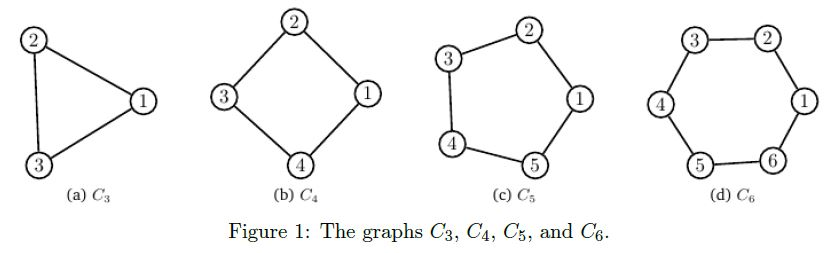
\includegraphics[width=\textwidth]{graficos/graph1}
\end{center} 

Your first step towards Nobel Prize fame is to be able to compute the number of matchings in the cycle graph $C_n$. In Figure 2 the seven matchings of the graph $C_4$ are depicted.

\begin{center}
	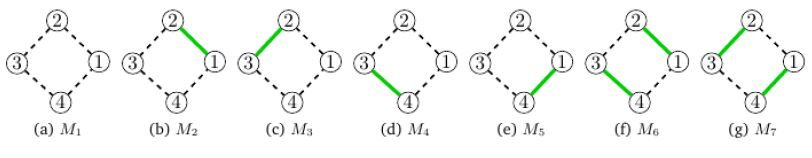
\includegraphics[width=\textwidth]{graficos/graph2}
\end{center} 

Figure 2: The matchings of $C_4$ . The edges that are part of the respective matching are coloured green, while the edges left out of the matching are dashed. $M_1 = 0$, $M_2 = \{ \{2,1\} \}$, $M_3 = \{ \{3,2\} \}$, $M_4 = \{ \{4,3\} \}$, $M_5 = \{ \{1,4\} \}$, $M_6 = \{ \{2,1\}, \{4,3\} \}$, and $M_7 = \{ \{3,2\}, \{1,4\} \}$.


\InputFile

For each test case, you get a single line containing one positive integer: $n$, with $3 \leq n \leq 10000$. \\


\OutputFile

For each test case, a row containing the number of matchings in $C_n$.  \\


\Example

\input ejemplos/edge.txt


URL:\\ 
http://uva.onlinejudge.org/index.php? \\
option=onlinejudge\&page=show\_problem\&problem=4521

\end{problema}
